% paper.tex

\NeedsTeXFormat{LaTeX2e}

\documentclass{jfp1}

\usepackage{float}
\usepackage{url}
\usepackage{listings}

\usepackage{tikz}
\usetikzlibrary{matrix}

\lstset{
  basicstyle=\ttfamily,
  columns=fullflexible,
  keepspaces=true,
  mathescape
}

%%% Macros for the guide only %%%
\providecommand\AMSLaTeX{AMS\,\LaTeX}
\newcommand\eg{\emph{e.g.}\ }
\newcommand\etc{\emph{etc.}}
\newcommand\bcmdtab{\noindent\bgroup\tabcolsep=0pt%
  \begin{tabular}{@{}p{10pc}@{}p{20pc}@{}}}
\newcommand\ecmdtab{\end{tabular}\egroup}
\newcommand\rch[1]{$\longrightarrow\rlap{$#1$}$\hspace{1em}}
\newcommand\lra{\ensuremath{\quad\longrightarrow\quad}}

\title[Automatically proving equivalence by type-safe reflection]
      {Automatically proving equivalence by type-safe reflection}

 \author[Franck Slama and Edwin Brady]
        {FRANCK SLAMA and EDWIN BRADY\\
         University of St Andrews, United Kingdom\\
         \email{fs39@st-andrews.ac.uk, ecb10@st-andrews.ac.uk}}

\jdate{December 2015}
\pubyear{2016}
\pagerange{\pageref{firstpage}--\pageref{lastpage}}
\doi{S0956796801004857}

\newtheorem{lemma}{Lemma}[section]

\begin{document}

\label{firstpage}

\maketitle

\begin{abstract}
% The abstract should be at most 300 words for the Journal of Functional Programming
Idris is a general purpose purely functional programming language with dependent types, aiming to bring type-based program verification techniques to functional programmers. One common difficulty with programming with dependent types is that proof obligations arise naturally once programs become even moderately sized. For example, implementing an adder for binary numbers indexed over their natural number equivalents will naturally lead to proof obligations for equalities of expressions over natural numbers. 
As far as possible, we would like to solve such proof obligations automatically. In this paper, we show one way to automate such proofs by reflection. We will show how representing Idris expressions in a reflected form, indexed by the original Idris expression, leads to straightforward construction and manipulation of proofs.
With this type-safe reflection technique, the resulting expressions are guaranteed to be faithful representations of the corresponding inputs and any generated proof is guaranteed to be a proof of the required property. 
We will first present the technique on a small example, where we aim to automatically prove equalities with universally quantified natural numbers and the associative addition operation, and will later show how this idea can be generalised to various kind of properties that might be available (for example, commutativity, distributivity, existence of neutral elements...), leading to a hierarchy of reflexive tactics for Monoids, Commutative Monoids, Groups, Commutative Groups, Rings, and so on, written in Idris, for proving different kind of equivalence. We will also show how each tactic reuses the other ones from the simplest structures, thus avoiding as much as possible the duplication of code.
\end{abstract}

%\tableofcontents

\section{Introduction}


One way to increase the confidence in the software we build is to formally prove its correctness using a proof assistant. Proofs assistants enable to write code, logical statements and proofs in the same language, and offer the guarantee that every proof will be automatically checked. Many of them are functional programming languages, like Coq~\cite{Bertot2004}, Idris~\cite{brady2013idris} and Agda~\cite{Norell2008}, and others, like the B-Method~\cite{Abrial1991} belong to the imperative paradigm. These different paradigms are internally supported by different logic. Systems like Coq, Idris and Agda are based on various higher order logics (CoC, a variant of ML and LUO respectively) and are realisations of the Curry-Howard correspondence, while the formal B method is based on Hoare logic. These different foundations lead to different philosophies and different ways to implement and verify a software, but all of them greatly increase the confidence of the produced software. However, these guarantees tend to be too often considered as perfect, when they are in fact far from it. Knuth was --certainly ironically-- saying ``Beware of bugs in the above code; I have only proved it correct, not tried it". The reality is precisely that a proof is not enough. When we prove the correctness of a function, we only gain the guarantee expressed by the proven lemma, and nothing more. 

Say we want to implement a formally verified sorting function for list of elements of type $T$, where $T$ is ordered by a relation $\leq$.
We can decide to define the sorting function with a ``weak" type, like $sort\ :\ List\ T\ \rightarrow\ List\ T$, and to use an external lemma to ensure the correctness of the function. Which property does this function has to respect? First, the output has to be sorted, so we need to define this notion of being sorted, here as an inductive predicate :

\begin{lstlisting}
data isSorted : {T:Type} -> (Order T) -> (List T) -> Type where
    NilIsSorted : (Tord : Order T) -> isSorted Tord []
    SingletonIsSorted : (Tord : Order T) -> (x:T) -> isSorted Tord [x]
    ConsSorted : {Tord : Order T} -> (h1:T) -> (h2:T) -> (t:List T) 
                 -> (isSorted Tord (h2::t)) -> (h1 $\leq$ h2) 
                 -> (isSorted Tord (h1::(h2::t)))
\end{lstlisting}
The first and second constructor of this predicate say that $[\ ]$ and $[x]$ are sorted according to any order, and for any $x$. The third one says that a list of two or more elements is sorted if $h1 \le h2$, and if the list deprived from its head is also sorted. In order to express that the result of $sort$ is sorted, we can prove the following lemma:
$sort\_correct : \forall\ (T:Type)\ (Tord:Order\ T)\ (l:List\ T),\ isSorted\ Tord\ (sort\ l)$. The problem with this specification is that it does not say anything about the content of the output. The function $sort$ could just return the empty list $[\ ]$ all the time, it would still be possible to prove this correctness lemma. Here, the problem is that the function is underspecified, and it is therefore possible to write a senseless implementation, which is unfortunately provably correct. Only a careful reader could realise that the lemma $sort\_correct$ forgets to mention that the input and output list should be in bijection, meaning that everything which was originally in the input list should still be in the output, and that nothing else should have been added.

Another bug in the specification could have been to simply forget the third constructor $ConsSorted$. But things more nasty can happen. Imagine that the third constructor of $isSorted$, called $consSorted$ would have been written with a typo, and that the condition $(h1 \leq h2) $ would have been incorrectly written as $(h1 \leq h1)$. Any list would be seen as ``sorted", just because of this single typo, and the algorithm could for example return its input unchanged. One could object that when doing the proof of correctness, we should realize that the proof is being done too easily, without having to use the essential property that the output is being built such as any element in the list is always lower or equal than its next element. The reality is quite different because many effort are going in the direction of proof automation, which aims to let the machine generate automatically the proof for some kind of goals. For example, Coq has already a Ring prover~\cite{coq2005} and many others automations, and Idris has been recently equipped with a hierarchy of provers for algebraics structures~\cite{Slama2016}. There are even extensions to languages, such as Ltac~\cite{DelahayeLTac} and Mtac~\cite{Ziliani13} that aim to help the automation of tactics. The problem is that the machine is never going to find a proof ``too easy", and will never report that something seems weird with the specification given by the user.

Thus, if we want to trust the proven software, we're now forced to believe that there is adequacy between the formal specification and the informal requirements. A switch has occurred. We used to have to trust code, but we now have to trust logical statements and predicates. But when the specification is too often as complicated as the code, why should we blindly believe in it, when we've first refused to blindly trust the code? The primary aim of this paper is to raise awareness of the adequacy concern, and to see how heterogeneous approaches, that mix both proofs and tests, can help to go a step forward in the certification process, in the context of proof assistants based on type theory.
More precisely, we :
\begin{itemize}
	\item Show some basic approaches to the problem of underspecification (section~\ref{sect:naiveApproaches})
	\item Present a new way to test the predicate in the proof assistant, by automatically generating terms, and we completely automate these tests (section~\ref{sect:testingInside})
	\item Present how we can go a step forward by replacing these tests about the predicate by some proofs (section~\ref{sect:aStepForward})
\end{itemize}

We use Idris, a dependently typed programming language, but all the ideas that we present here can be applied to any proof assistant based on type theory. The running example that we use in this paper can be found online at \url{https://github.com/FranckS/}.




\section{A Simplified Problem: Proving Equalities with Natural Numbers and Additions}

\label{sect:ideas}

We will first present the basic ideas of our technique on a simplified problem, in which we aim to deal with universally quantified natural numbers and additions.
For example, we would like to be able to automatically generate proofs of goals like $\forall x1\ x2\ x3:Nat,\ (x1 + l2) + (x3 + x4) = (x1 + (x2 + x3)) + x4$ [Example 1]. \\
For this smaller problem, we have decided to only work with the associativity of $+$ : $plusAssociative : \forall x1\ x2\ x3,\ (x1 + x2) + x3 = x1 + (x2 + x3)$ and with the fact that Z is a right neutral element for the $+$ operation : $plusZeroRightNeutral : \forall x, x + Z = x$. Note that $Z$ is also a left neutral element, but this property is not needed because we have this behaviour by reduction, as $+$ is defined recursively on its first argument. Of course, some datatypes can have more or less properties than these two, and this work will be extended in sections 3 and 4 where we will present a very general hierarchy of provers for multiple algebraic structures. \\
Thus, in definitive, in this section, we want to write a decision procedure, able to tell if two expressions composed of universally quantified natural numbers and additions of these numbers are equal, and to produce a proof of this equality if appropriate, where ``equal" has the meaning syntactically equal or equal thanks to the associativity and right neutral properties.


\subsection{Working by reflection}

When trying to prove this kind of equalities, the variables are abstracted, and they become part of the context. On the example 1 just above, after abstraction of the variables, the goal becomes simply $(x1 + x2) + (x3 + x4) = (x1 + (x2 + x3)) + x4$, which is something of the general form $x=y$.
The general idea --that will also apply for the more general problem detailed in the next sections-- will be to normalize both sides of the "potential equality" $x=y$, and afterwards to compare them using Leibniz syntactical equality.
The goal of the normalization is to compute a canonical representation for a number $x$, such that any other number provably equal to $x$ (by using the two available properties) will have the same canonical representation. For example, the normalisation might transform $x+((y+Z)+z)$ into $(x+y)+z$ if we decide that the normal form will be completely left associative, and that every addition between an element $a$ and zero should be simplified to $a$. It will then be possible to decide the equality by simply comparing the normalised left and right hand sides with a simple and strict syntactical equality. This is in fact what we do all the time when we have to decide if two things, written differently, are equal or not. When a human is given two mathematical polynomials and has to decide the equality of these functions, a technique that always works is to decide once and for all a canonical representation of polynomials, and to put both polynomials in this form. If the normalised forms are the same, then the two original polynomials are equal, otherwise they do not represent the same computation.\\
\\
In fact, such a normalisation function can't be written directly, because in the LHS and RHS of $x=y$, we potentially have variables which have been universally quantified. And the normalization function needs to do different treatments for a ``variable natural number" (a number which has been universally quantified) and for the constant $Z$. This is not possible yet, because once the variables are abstracted, they are just ordinary values of type $Nat$, and there is no way to distinguish them. Indeed, this information only exists at the level of the ASTs representing the two terms, and we do not have a direct access to these syntax trees.
For this reason, we will work by reflection. In this little example, it means that we will define a datatype that will be used as an encoding of natural numbers, or more precisely, an encoding of natural numbers composed of ``variable numbers", $Z$, and additions of these things. This datatype will let us inspect the internal structure of a number by pattern matching.
Previously, we were only able to pattern match a natural number against the constructors $Z$ and $S$, which wasn't what we needed.  With the first approximation of the data type $Expr$ presented in the figure~\ref{reflectedNaturalNumbers0}, we will be allowed to pattern match an encoding of number against the constructors $Plus$, $Var$ and $Zero$.


\begin{figure}[H]
\figrule
\begin{center}
\begin{lstlisting}
data Expr : ($\Gamma$ : Vect n Nat) $\rightarrow$ Type where
     Plus : {n:Nat} $\rightarrow$ {$\Gamma$:Vect n Nat} $\rightarrow$ 
            Expr $\Gamma$ $\rightarrow$ Expr $\Gamma$ $\rightarrow$ Expr $\Gamma$
     Var  : {n:Nat} $\rightarrow$ {$\Gamma$:Vect n Nat} $\rightarrow$ 
            (i : Fin n) $\rightarrow$ Expr $\Gamma$
     Zero : {n:Nat} $\rightarrow$ ($\Gamma$:Vect n Nat) $\rightarrow$ 
            Expr $\Gamma$ Z
\end{lstlisting}
\end{center}
\caption{First version of reflected natural numbers}
\label{reflectedNaturalNumbers0}
\figrule
\end{figure}


Variables are represent using a De Brujin-like index : (Var FZ) denotes a variable, (Var (FS FZ)) another one, and so on.

The type Expr is indexed over a vector of numbers $\Gamma$, which is the context of all universally quantified variables. In the example 1, we will encode $(x1 + x2) + (x3 + x4)$ and $(x1 + (x2 + x3)) + x4$ in a context where four elements are present. The first element of this context denotes the variable $x1$, the second denotes $x2$, and so on.
Thus, the left hand side will be encoded by :

\begin{figure}[H]
\figrule
\begin{center}
\begin{lstlisting}
e1 : (x, y, z : Nat) $\rightarrow$ 
           Expr [x, y, z]
e1 x y z = Plus (Plus (Var FZ) (Var (FS FZ))) 
                (Plus (Var FZ) (Var (FS (FS FZ))))
\end{lstlisting}
\end{center}
\caption{Reflected LHS with the first version of reflected numbers showed in \ref{reflectedNaturalNumbers0}}
\figrule
\end{figure}

\subsection{Type safe reflection}

If we continue with this first definition of $Expr$, the normalisation function will certainly take an Expr and produce another Expr, and we will need to prove the following correctness lemma afterwards : \\
$\forall\ e:Expr\ \Gamma,\ reify\ (reduce\ e)\ =\ reify\ e$ \\
where $reify$ is a function computing the interpretation of an Expr in a context $\Gamma$, that is to say, the natural number that this Expr is encoding.
This proof can be quite tricky to build because it relies on the complete behaviour of the reduction and on the way the interpretation is computed.
For this little example, the reduction procedure won't be too heavy, but in the next sections, with more sophisticated algebraic structures, we will have more properties to deal with and it will certainly become more problematic to unfold the definition of a gigantic reduction procedure. We want to avoid pain as much as possible, and for this reason, we don't want to have to write big proofs, and even to avoid the writing of proofs as much as possible. \\
\\
To avoid this source of complexity, we add an index to the type $Expr$, and this index is precisely the concrete number that the Expr is encoding. This is the first brick to our type-safe reflection mechanism. Thus, it won't be necessary to define the $reify$ function, as we will know directly the concrete element reflected by a term of type $Expr\ \Gamma\ x$ just by looking at its index $x$. We also get the guarantee that the reflection of an expression $e$ is indeed a faithful representation of $e$ \\

\begin{figure}[H]
\figrule
\begin{center}
\begin{lstlisting}
using (x : Nat, y : Nat, $\Gamma$ : Vect n Nat)
  data Expr : (Vect n Nat) $\rightarrow$ Nat $\rightarrow$ Type where
       Plus : Expr $\Gamma$ x $\rightarrow$ Expr $\Gamma$ y $\rightarrow$ 
              Expr $\Gamma$ (x + y)
       Var  : (i : Fin n) $\rightarrow$ Expr $\Gamma$ (index i $\Gamma$)
       Zero : Expr $\Gamma$ Z
\end{lstlisting}
\end{center}
\caption{Second version of reflected number with embedded denotation}
\label{reflectedNaturalNumbers}
\figrule
\end{figure}

For an expression $ex\ :\ Expr\ \Gamma\ x$, we will say that ``$ex$ denotes (or encodes) the number $x$ in the context $\Gamma$".
When an expression is a variable, the denoted number is simply the corresponding variable in the context, ie, $(index\ i\ \Gamma)$.
Also, the $Zero$ expression denotes the natural number $Z$.
Finally, if $ex$ is an expression encoding the number $x$, and $ey$ is an expression encoding the number $y$, then the expression $Plus\ ex\ ey$ denotes the concrete number $(x + y)$.


\subsection{A correct by construction approach}

We want to write the reduction function on a ``correct by construction" way, which means that no additional proof should be required after the definition of the function. Thus, $reduce$ will produce the proof that the new Expr freshly produced has the same interpretation as the original Expr, and this will be made easier by the fact that the data type Expr is now indexed over the real --concrete-- number : a term of type $Expr\ \Gamma\ x$ is the encoding of the number $x$.
Thus, we can write the type of $reduce$ like this : \\
$reduce\ :\ Expr\ \Gamma\ x\ \rightarrow\ (x'\ **\ (Expr\ \Gamma\ x',\ x\ =\ x'))$ \\
The function $reduce$ produces a dependent pair : the new concrete number $x'$, and a pair made of an $Expr\ \Gamma\ x'$ which is the new encoded term indexed over the new concrete number we have just produced, and a proof that old and new --concrete-- numbers are equal.
Note that this function can't simply produce an $Expr\ \Gamma\ x$, because the concrete number on which the resulting expression will be indexed is not necessary syntactically equal to the original number since this equality can use the two available properties. Said differently, even if we can prove $x=x'$ (if the function is correctly defined), we do not have $x \equiv x'$.
And in fact, what really interests us in this function is precisely this proof of $x\ =\ x'$.
The reason is that when we try to automatically prove $x=y$, these proofs will be the crucial part for the construction of the desired proof. \\
\\
The tactic will work as follow.
We have an expression $ex$ encoding $x$, and an expression $ey$ encoding $y$. We will normalize $ex$, and this will give a new concrete number $x'$, a new expression $ex':Expr\ \Gamma\ x'$, and a proof of $x=x'$. We will do the same with $ey$, and we will get a new concrete number $y'$, an expression $ey':Expr\ \Gamma\ y'$, and a proof of $y=y'$. \\
It is now enough to simply compare $ex'$ and $ey'$ using a standard syntactical equality because these two expressions are now supposed to be in normal form :

\begin{figure}[H]
\figrule
\begin{center}
\begin{lstlisting}
eqExpr : (e : Expr $\Gamma$ x) $\rightarrow$ (e' : Expr $\Gamma$ y) $\rightarrow$ Maybe (e = e')
eqExpr (Plus x y) (Plus x' y') with (eqExpr x x', eqExpr y y')
  eqExpr (Plus x y) (Plus x y) | (Just Refl, Just Refl) = Just Refl
  eqExpr (Plus x y) (Plus x' y') | _ = Nothing
eqExpr (Var i) (Var j) with (decEq i j)
  eqExpr (Var i) (Var i) | (Yes Refl) = Just Refl
  eqExpr (Var i) (Var j) | _ = Nothing
eqExpr Zero Zero = Just Refl
eqExpr _ _ = Nothing
\end{lstlisting}
\end{center}
\caption{Syntactical equality between reflected terms}
\label{syntacticalEq}
\figrule
\end{figure}


Now, if the two normalised expressions $ex'$ and $ey'$ are equal, then they necessary have the same type\footnote{We are working with the heterogeneous equality JMeq by default in Idris, but as always, the only way to have a proof of a:A = b:B is when A=B}, and therefore $x'=y'$.
By rewriting the two equalities $x=x'$ and $y=y'$ (that we obtained during the normalisations) in the new equality $x'=y'$, we can get a proof of $x=y$. This is what the function $buildProof$ is doing.

\begin{figure}[H]
\figrule
\begin{center}
\begin{lstlisting}
buildProof : {x : Nat} $\rightarrow$ {y : Nat} $\rightarrow$ Expr $\Gamma$ x' $\rightarrow$ Expr $\Gamma$ y' 
           $\rightarrow$ (x = x') $\rightarrow$ (y = y') $\rightarrow$ Maybe (x = y)
buildProof ex' ey' lp rp with (eqExpr ex' ey')
  buildProof ex' ex' lp rp | Just Refl = ?MbuildProof
  buildProof ex' ey' lp rp | Nothing = Nothing
\end{lstlisting}
\end{center}
\caption{Building the desired proof with the two proofs of equality}
\label{buildProof}
\figrule
\end{figure}

The argument of type $Expr\ \Gamma\ x'$ is the normalised reflected left hand size of the equality, which represents the value $x'$. Before the normalisation, the reflected LHS was reflecting the value $x$. The $Expr\ \Gamma\ y'$ is the normalised reflected right hand size, which now represents the value $y'$, but which was encoding $y$ before the normalisation. The function also expects the proofs that $x=x'$ and $y=y'$, and we should be able to pass them because the normalisation function has also produced the proof of equality between the original and the new concrete values.

As mentioned, the proof for the metavariable $MbuildProof$ is just a rewriting of the two equalities :

\begin{figure}[H]
\figrule
\begin{center}
\begin{lstlisting}
  MbuildProof = proof {
  intros; refine Just; rewrite sym p1; rewrite sym p2; exact Refl;
}  
\end{lstlisting}
\end{center}
\caption{buildProof metavariable}
\label{MbuildProof}
\figrule
\end{figure}

Finally, the main function which tries to prove the equality $x=y$ simply has to reduce the two reflected terms encoding the left and the right hand side, and to use the function $buildProof$ in order to compose the two proofs that we just obtained :

\begin{figure}[H]
\figrule
\begin{center}
\begin{lstlisting}
  testEq : Expr $\Gamma$ x $\rightarrow$ Expr $\Gamma$ y $\rightarrow$ Maybe (x = y)
  testEq ex ey = 
     let (x' ** (ex', px)) = reduce ex in 
     let (y' ** (ey', py)) = reduce ey in
        buildProof ex' ey' px py 
\end{lstlisting}
\end{center}
\caption{testEq}
\label{testEq}
\figrule
\end{figure}

We now need to define the function reduce. To do that, we have to decide a canonical representation of associative natural numbers. We decide that the left associative form will be the canonical representation. Thus, the $reduce$ function has to rewrite the reflected terms by rearranging the parentheses in order to transform the underlying concrete number in the form $(...((x1 + x2) + x3) ... + xn)$. To do so, one possibility is to define a new datatype which captures this property, and to write a function going from $Expr$ to this new type. Thus it will be easier to be certain that we are effectively computing the normal form : forcing properties to hold by the shape of a datatype is a good usage of dependent types when, like here, it doesn't introduce more complications.

\begin{figure}[H]
\figrule
\begin{center}
\begin{lstlisting}
data LExpr : ($\Gamma$ : Vect n Nat) $\rightarrow$ Nat $\rightarrow$ Type where
     LPlus : LExpr $\Gamma$ x $\rightarrow$ (i : Fin n) 
             $\rightarrow$ LExpr $\Gamma$ (x + index i $\Gamma$)
     LZero : LExpr $\Gamma$ Z
\end{lstlisting}
\end{center}
\caption{Reflected left associative numbers}
\label{LExpr}
\figrule
\end{figure}

This datatype has only two constructors. In fact, it combines the previous $Var$ and $Plus$ constructors so that it becomes impossible to write an expression which isn't left associative (because LPlus is only recursive on its first argument).
 
As part of the normalization, we write a function $expr\_l$ which converts an $Expr\ \Gamma\ x$ to a $LExpr\ \Gamma\ x'$ and which produces a proof of $x=x'$. This function will therefore use the two available properties multiple times, while rewriting the term until the fully left associative desired form is obtained.

\begin{figure}[H]
\figrule
\begin{center}
\begin{lstlisting}
expr_l : Expr $\Gamma$ x 
         $\rightarrow$ (x' ** (LExpr $\Gamma$ x', x = x'))
expr_l Zero = (_ ** (LZero, Refl))
expr_l (Var i) = (_ ** (LPlus LZero i, Refl))
expr_l (Plus ex ey) = 
  let (x' ** (ex', px)) = expr_l ex in
  let (y' ** (ey', py)) = expr_l ey in
  let (res ** (normRes, Pres)) = plusLExpr ex' ey' in
    (res ** (normRes, rewrite px in (rewrite py in Pres)))
      where 
      plusLExpr : {$\Gamma$ : Vect n Nat} $\rightarrow$ {x, y : Nat} 
            $\rightarrow$ LExpr $\Gamma$ x -> LExpr $\Gamma$ y  
            $\rightarrow$ (z ** (LExpr $\Gamma$ z, x+y=z))
      plusLExpr {x=x} ex LZero =
        (_ ** (ex, rewrite (plusZeroRightNeutral x) in Refl))            
      plusLExpr ex (LPlus e i) =
        let (xRec ** (rec, prfRec)) = plusLExpr ex e in
            (_ ** (LPlus rec i, ?MplusLExpr))

\end{lstlisting}
\end{center}
\caption{Production of the left associative form}
\label{expr_l}
\figrule
\end{figure}
In the case of an addition $Plus\ ex\ ey$, the function $expr\_l$ does the job of normalisation recursively on $ex$ and on $ey$, and then it uses the sub-function $plusLExpr$ to normalise the addition of these two --already normalised-- terms. This sub-function $plusLExpr$ has two kind of simplifications to do. When the second argument is an $LZero$, it simply returns its first arguments along with the justification for this rewriting, which obviously uses $plusZeroRightNeutral$. However, when the second argument is an $LPlus\ e\ i$, it continues recursively by computing $plusLExpr\ ex\ e$, and it finally adds $i$ to it. That had for effect to move the parenthesis on the left, and this treatment is going to be justified during the proof of the meta variable $MplusLExpr$ by the use of $plusAssociative$.

This metavariable $MplusLExpr$ requires us to prove the goal : $x1 + (x2 + index\ i\ \Gamma) = xrec + index\ i\ \Gamma$ in a context where we've got, amongst other things, $prfRec : x1 + x2 = xrec$.
By using the property of associativity on the goal, we now need to prove $(x1 + x2) + index\ i\ \Gamma$, which can be done by rewriting the proof $prfRec$ obtained recursively.

\begin{figure}[H]
\figrule
\begin{center}
\begin{lstlisting}
MplusLExpr = proof {
  intros
  rewrite (sym (plusAssociative x1 x2 (index i $\Gamma$))); rewrite prfRec; 
  exact Refl;
}
\end{lstlisting}
\end{center}
\caption{Proof of the metavariable MplusLExpr}
\label{MplusExpr}
\figrule
\end{figure}

It is really important to understand that the root of the automatic building of the desired proof of $x=y$ happens precisely in these nested use of $plusZeroRightNeutral$ and $plusAssociative$ that we've seen in the definition of $expr\_l$ and of its meta-variable $MplusLExpr$. These proofs replace the arithmetical proofs that we were doing previously by hand, as it was the case in section 1 with the lemma $adc\_lemma\_2$. \\
\\
Using this new datatype $LExpr$ has changed the representation of our encoded lists, so we need to convert back an $LExpr\ \Gamma\ x$ to an $Expr\ \Gamma\ x$. The function $l\_expr$ does this easy task.
\begin{figure}[H]
\figrule
\begin{center}
\begin{lstlisting}
l_expr : LExpr $\Gamma$ x $\rightarrow$ Expr $\Gamma$ x
l_expr LZero = Zero
l_expr (LPlus x i) = Plus (l_expr x) (Var i)
\end{lstlisting}
\end{center}
\caption{Going back from LExpr to Expr}
\label{l_expr}
\figrule
\end{figure}


We notice that in order to transform the expression into its left associative equivalent representation, we've effectively needed to know where the variables and the $Z$ constants are : the functions $expr\_l$ and $l\_expr$ are doing different treatments for these two possibilities. \\
\\

We can now define the reduction, which is just the composition of the two previous functions $expr\_l$ and $l\_expr$:

\begin{figure}[H]
\figrule
\begin{center}
\begin{lstlisting}
  reduce : Expr $\Gamma$ x $\rightarrow$ (x' ** (Expr $\Gamma$ x', x = x'))
  reduce e = 
     let (x' ** (e', prf)) = expr_l e in
         (x' ** (l_expr e', prf))
\end{lstlisting}
\end{center}
\caption{Reduction function}
\label{reduce}
\figrule
\end{figure}


At the moment, what we've got is not exactly a real tactic, in the sense that we only have a function which produces a value of type $Maybe (x = y)$. A real tactic would be a wrapper of this function that could properly fail with an error message when the two terms are not equal. However, here, when $x\ne y$, the function $testEq$ will simply produce the value $Nothing$. \\

\subsection{Usage of the ``tactic"}

It's now time to see how to use this minimalist ``tactic".
Let's define two expressions $e1$ and $e2$, respectively representing the numbers $((x + y) + (x + z))$ and $(x + ((y + x) + z))$ in the context $[x, y, z]$ of three abstracted variables.


\begin{figure}[H]
\figrule
\begin{center}
\begin{lstlisting}
e1 : (x, y, z : Nat) 
    $\rightarrow$ Expr [x, y, z] ((x+y) + (x+z))
e1 x y z = Plus (Plus (Var FZ) 
                      (Var (FS FZ))) 
                (Plus (Var FZ) 
                      (Var (FS (FS FZ))))

e2 : (x, y, z : Nat) 
     $\rightarrow$ Expr [x, y, z] (x + ((y + x) + z))
e2 x y z = Plus (Var FZ) 
                (Plus (Plus (Var (FS FZ)) 
                            (Var FZ)) 
                      (Var (FS (FS FZ))))
\end{lstlisting}
\end{center}
\caption{Two test expressions}
\label{e1_e2}
\figrule
\end{figure}

The numbers denoted by the expressions $e1$ and $e2$ are equal, and we can generate a proof of this fact by using $testEq$.

\begin{figure}[H]
\figrule
\begin{center}
\begin{lstlisting}
e1_e2_testEq : (x, y, z : Nat) 
             $\rightarrow$ Maybe (((x + y) + (x + z)) = (x + ((y + x) + z)))
e1_e2_testEq x y z = testEq (e1 x y z) (e2 x y z)
\end{lstlisting}
\end{center}
\caption{Generating automatically the desired proof}
\label{e1_e2_testEq}
\figrule
\end{figure}


And if we ask for the evaluation of this term, we should obtain $Just$ and a proof of equality between the two underlying numbers.

\begin{figure}[H]
\figrule
\begin{center}
\begin{lstlisting}
#\x => \y => \z => e1_e2_testEq x y z

\x => \y => \z => Just (replace (sym (replace (sym (replace 
(sym (plusAssociative x 0 y)) (replace (replace (sym 
(plusZeroRightNeutral x)) Refl) Refl))) (replace (sym 
(replace (sym (plusAssociative x 0 z)) (replace (replace 
(sym (plusZeroRightNeutral x)) Refl) Refl))) (replace (sym 
(plusAssociative (x+y) x z)) [...]
: (x : Nat) -> (y : Nat) -> (z : Nat) 
  -> Maybe ((x + y) + x + z 
            = x + (y + x) + z)
\end{lstlisting}
\end{center}
\caption{Obtained proof}
\label{obtainedProof}
\figrule
\end{figure}

And we effectively get the proof of equality we wanted. As expected, this proof uses the properties of associativity ($plusAssociative$) and the property of neutrality of $Z$ for $+$ ($plusZeroRightNeutral$).


\subsection{Construction of the reflected terms}
\label{sect:ReflectNat}

For the moment, even if what we have is perfectly usable and works, we had to create these encodings $e1$ and $e2$ by hand, which is easy but time consuming. We have replaced the (potentially hard) problem of proving something by the simplest problem of simply creating some encodings. This is already a huge simplification, because as it can be seen in the definitions of $e1$ and $e2$, the reflected terms completely follow the structure of the expression to encode : there's absolutely no creativity needed for this task, unlike the proving activity. The way to create the encodings is in fact so systematic that, of course, we would like to automatize it in order to get a real and completely automatic tactic.

However, we can also note that even when done by hand, there is no room for making mistakes in this simple task of encoding : we simply can't generate a wrong encoding : if $e1$ and $e2$ are not respectively reflecting $((x+y) + (x+z))$ and $(x + ((y + x) + z))$ then these definitions won't typecheck because the expected and real index won't match.

We still want an automatic way of constructing these reflected terms because what we have so far is enough to demonstrate that our prover works, but that's not yet enough for being used intensively. We want to program an automatic way of going from the concrete values (of type $Nat$), to the reflected terms (of type $Expr$). The only way to do that is to inspect the abstract syntax tree of the concrete value.
By using Idris's reflection mechanism, we can tag a function with the keyword "\%reflection", which means that this function runs on syntax instead of values. 

\begin{figure}[H]
\figrule
\begin{center}
\begin{lstlisting} [mathescape]
%reflection
total
reflectNat : {n:Nat} $\rightarrow$ ($\Gamma$ : Vect n Nat) $\rightarrow$ (x:Nat) 
             $\rightarrow$ (m ** ($\Gamma'$ : Vect m Nat ** (Expr ($\Gamma$ ++ $\Gamma'$) x)))
\end{lstlisting}
\end{center}
\caption{Type of the function for reflecting natural numbers}
\label{reflectNatType}
\figrule
\end{figure}

This function will reflect the natural number $x$ in the context of $\Gamma$, which contains $n$ already abstracted variables. This function will compute an extension --of arbitrary size $m$-- to the context, called $\Gamma'$. This extension will contain the variables used in $x$ that weren't already present in $\Gamma$. It will also produce the reflected term, which is expressed in the complete context $\Gamma ++\ \Gamma'$, and which is, of course, indexed over the concrete value $x$.

If $x$ is the natural number $Z$, then we don't have any variable to add to $\Gamma$, so the extension will be the empty vector, and the reflected expression is simply $Zero$.

 \begin{figure}[H]
\figrule
\begin{center}
\begin{lstlisting} [mathescape]
reflectNat {n=n} G Z = (Z ** ([] ** (Zero {n=n+0} {G=G++[]})))
\end{lstlisting}
\end{center}
\caption{Reflecting natural numbers - pattern for zero}
\label{reflectNat_pattern1}
\figrule
\end{figure}

If the natural number to reflect is an addition $x+y$, then we will start by reflecting $x$ in the context of $\Gamma$. That will give us an extension $\Gamma'$ and an expression $ex$ of type $Expr\ (\Gamma ++\ \Gamma')\ x$. We continue by reflecting $y$, but this time in the context $(\Gamma ++\ \Gamma')$ of $n+m$ already abstracted variables, because the reflection of $x$ has potentially abstracted some new variables, and we don't want to abstract them a second time. That will give us a second extension $\Gamma''$ and an expression $ey$ of type $Expr\ ((\Gamma ++\ \Gamma')\ ++\ \Gamma'')\ y$. We now simply want to return the $Plus$ of $ex$ and $ey$, but we can't immediately, because these encodings aren't defined on the same context. The context in which $ex$ makes sense is $(\Gamma ++\ \Gamma')$, but the context in which $ey$ makes sense is $((\Gamma ++\ \Gamma')\ ++\ \Gamma'')$. We will therefore need a function of weakening that takes a reflected expression $ex$, and returns the same expression, but expressed in an augmented context.

 \begin{figure}[H]
\figrule
\begin{center}
\begin{lstlisting} [mathescape]
reflectNat $\Gamma$ (x + y) =
     let (_ ** ($\Gamma'$ ** ex)) = (reflectNat $\Gamma$ x) in
     let (_ ** ($\Gamma''$ ** ey)) = (reflectNat ($\Gamma$ ++ $\Gamma'$) y) in
     let result = Plus (weaken $\Gamma''$ ex) ey in 
        (_ ** (($\Gamma'$ ++ $\Gamma''$) ** ?MreflectNat_1))
\end{lstlisting}
\end{center}
\caption{Reflecting natural numbers - pattern for a plus}
\label{reflectNat_pattern2}
\figrule
\end{figure}

The total extension that has been computed is $\Gamma' ++\ \Gamma''$, and the metavariable $MreflectNat\_1$ simply uses the associativity of the append operation to prove that the provided context $((\Gamma ++\ \Gamma')\ ++\ \Gamma'')$ is equal to the expected one $(\Gamma ++\ (\Gamma'\ ++\ \Gamma''))$. \\
\\
The function $weaken$ is easy to write because we're adding the extension $\Gamma'$ on the right of $\Gamma$. For example, extending the context $[v,\ w,\ x]$ with $[y,\ z]$ produces the context $[v,\ w,\ x,\ y,\ z]$. The variables $v$, $w$ and $x$, which were refereed to as the first, second and third variables in $\Gamma$, are still the first, second and third variables in the complete context. That means that a variable $Var\ i$ will still be a $Var\ i$, the position $i$ hasn't changed by augmenting the context.

 \begin{figure}[H]
\figrule
\begin{center}
\begin{lstlisting} [mathescape]
weaken : {n:Nat} $\rightarrow$ {m:Nat} $\rightarrow$ {$\Gamma$:Vect n Nat} $\rightarrow$ {x:Nat} 
          $\rightarrow$ ($\Gamma'$:Vect m Nat) $\rightarrow$ (Expr $\Gamma$ x) $\rightarrow$ (Expr ($\Gamma$ ++ $\Gamma'$) x)
weaken $\Gamma'$ Zero = Zero
weaken $\Gamma'$ (Plus e1 e2) = Plus (weaken $\Gamma'$ e1) (weaken $\Gamma'$ e2)
weaken {n=n} {m=m} {$\Gamma$=$\Gamma$} $\Gamma'$ (Var i) = Var (convertFin _ i m)    
\end{lstlisting}
\end{center}
\caption{Weakening function}
\label{weaken}
\figrule
\end{figure}


The position $i$ hasn't changed but however, the original $i$ had type $Fin\ n$, but the new $i$ must have type $Fin\ (n+m)$. This is why we've used $convertFin$, which returns the same element, but seen in a bigger $Fin$.

 \begin{figure}[H]
\figrule
\begin{center}
\begin{lstlisting} [mathescape]
convertFin : (n:Nat) $\rightarrow$ (i:Fin n) $\rightarrow$ (x:Nat) $\rightarrow$ Fin (n+x)
\end{lstlisting}
\end{center}
\caption{Conversion of a Fin}
\label{convertFin}
\figrule
\end{figure}

We've treated the case of the constant $Z$ and the case of the addition. We now have to deal with the last possibility of a variable. For encoding a variable, we must see if this variable is already present in the context $\Gamma$ of already abstracted variables. If it is already present there, then there is no extension to build, and the reflected term is simple $Var\ (convertFin\ n\ i\ Z)$, where $i$ is the position of the variable in this context $\Gamma$. The conversion was needed because the original context was $\Gamma$, and the new one is $(\Gamma ++\ [\ ])$, which aren't automatically unifiable. However, if if this variable is missing, then we should add it, which means that we will return an extension containing this single variable. The original context $\Gamma$ had a size of $n$, and we've built an extension of size one, so the complete context has therefore size $(n+1)$. The variable that we've added is currently the last one of these  $(n+1)$ variables. If we use a function\footnote{This function doesn't have the type $(n:Nat)\ \rightarrow Fin\ n$ because there is no last element of a $Fin$ of size zero as there's no element at all}  $lastElement'\ :\ (pn:Nat)\ \rightarrow\ Fin\ (pn+1)$ to construct the last element of a $Fin$ of size $pn+1$, then the reflected term that we need to produce is simply $Var\ (lastElement'\ n)$. 

 \begin{figure}[H]
\figrule
\begin{center}
\begin{lstlisting} [mathescape]
reflectNat {n=n} $\Gamma$ t with (isElement t $\Gamma$)
  | Just (i ** p) = let result = Var {$\Gamma$=$\Gamma$++[]} (convertFin n i Z) in
                        (Z ** ([] ** ?MreflectNat_2))
  | Nothing ?= (((S Z) ** ([t] ** Var {$\Gamma$=$\Gamma$++[t]} (lastElement' n))))  
            
\end{lstlisting}
\end{center}
\caption{Reflecting natural numbers - pattern for a variable}
\label{reflectNat_pattern3}
\figrule
\end{figure}

$isElement$ is the function which checks whether an element $x$ belongs to a vector $\Gamma$, and if so, returns $Just$ and a dependent pair containing the index of $x$ in this vector, and a proof that $index\ i\ \Gamma\ =\ x$.

 \begin{figure}[H]
\figrule
\begin{center}
\begin{lstlisting} [mathescape]
isElement : {n:Nat} $\rightarrow$ (x : a) $\rightarrow$ ($\Gamma$ : Vect n a) 
            $\rightarrow$ Maybe (i:Fin n ** (index i $\Gamma$ = x))
\end{lstlisting}
\end{center}
\caption{Returns the index and the proof that this index is the right one}
\label{isElement}
\figrule
\end{figure}

The metavariable $MreflectNat\_2$ will require us to prove that the provided term of type $Expr\ (\Gamma ++\ [\ ])\ (index\ (convertFin\ n\ i\ Z)\ (\Gamma ++\ [\ ]))$ is transformable into a term of the expected type $Expr\ (\Gamma ++\ [\ ])\ t$. This is doable by using the proof $p$ --returned by $isElement$-- which says that $index\ i\ \Gamma\ =\ t$, together with the fact that $convertFin$ does not change the index, but only converts its type.

As for the case where $t$ wasn't in the original context (the $Nothing$ case), we will need to prove that we can convert $(index\ (lastElement'\ n)\ (\Gamma ++\ [t]))$ into $t$. This is doable because we can prove the lemma $elemInBigerVect\ :\ \{T:Type\}\ \rightarrow \{v:Vect\ n\ T\} \rightarrow (i:Fin\ n) \rightarrow (elem:T) \rightarrow (proofInside : index\ i\ v\ =\ elem) \rightarrow (head:T) \rightarrow (index\ (FS\ i)\ (head::v)\ =\ elem)$.
            
That finishes the automatic reflection for this specific prover. The encoding of $((x+y) + (x+z))$ can now be produced automatically with $reflectNat\ [\ ]\ ((x+y)\ +\ (x+z))$.
            

            



\section {Back to the general problem : A hierarchy of tactics}

Now that we have introduced our ideas on this little example, it is time to apply them for our main goal, more general : the implementation of a hierarchy of tactics proving equalities in algebraic structures. Very often, the properties available on a given type are the ones of a well known algebraic structure, like semi-group, monoid, group, ring...  We will no longer only work with the properties of associativity and of right neutral element for natural numbers as it was the case in the previous section, but we will have available the properties of different structures, and these tactics will be usable for any type that satisfies these properties.

We will construct a hierarchy of type classes and will write one tactic for each of these type class. All our tactics (the ring prover, the group prover...) will be able to work on any type, being given that an instance of the corresponding type class is provided.

\subsection {Hierarchy of type classes}

In fact, we don't only want to be able to prove equalities, but more generally equivalence. We want to give the user the possibility to define his own equivalence notion, assuming he's able to provide the properties of the structure he wants to use. This equivalence relation on $c$ has the following profile $(\simeq) : c \rightarrow y \rightarrow Type$\footnote{This 'Type' would be a 'Prop' in systems --like Coq-- that make a distinction between the world of computations and the world of logical statements}, and has to be accompanied by the usual properties of reflexivity, symmetry and transitivity.

All of our tactics will require to have a way of testing this equivalence between elements of the underlying set, that is to say, a way to test equivalence between constants. For this reason, we define a notion of "set", which only requires the definition of the equivalence relation --accompanied with the proofs that this is indeed an equivalence relation-- and this equivalence test $set\_eq$. All the algebraic structures will later extend this type class :

\begin{figure}[H]
\figrule
\begin{center}
\begin{lstlisting}
class Set c where
    ($\simeq$) : c -> c -> Type

    refl : (x:c) -> x $\simeq$ x
    sym : {x:c} -> {y:c} -> (x $\simeq$ y) -> (y $\simeq$ x)
    trans : {x:c} -> {y:c} -> {z:c} -> (x $\simeq$ y) -> (y $\simeq$ z) -> (x $\simeq$ z)    
    
    set_eq : (x:c) -> (y:c) -> Maybe (x $\simeq$ y)
\end{lstlisting}
\end{center}
\caption{Set}
\figrule
\end{figure}
If the user wants to prove propositional equalities, then he will simply instantiate $(\simeq)$ with the built-in $(=)$ during the definition of the instance of $Set$.
Note that $(\simeq)$ is only weakly decidable in the sense that $set\_eq$ only produces a proof when the two elements are equivalent, but it doesn't produce a proof of dis-equivalence when they are different -- instead, it simply produces the value $Nothing$--. That's quite natural, since we want to generate proof of equivalence, and not to generate counter examples for proving dis-equivalence, which is another problem.

Obviously, there is no tactic associated to $Set$, since we have no operations and no properties associated to this structure. Therefore, equivalence in a $Set$ are just the "syntactical equivalence", and they can simply be proven with $refl$.
The first real structure, almost trivial, is the magma. A magma has just a $Plus$ operation, and no properties about it.

\begin{figure}[H]
\figrule
\begin{center}
\begin{lstlisting}
class Set c => Magma c where
    Plus : c -> c -> c
\end{lstlisting}
\end{center}
\caption{Magma}
\figrule
\end{figure}

This code means that a type $c$ (for $carrier$) is a Magma if it is already a Set (ie, it is equiped with the equivalence relation $\simeq$ and the test $set\_eq$), and if it has a $Plus$ operation.
In fact, all operations, like the Plus here, need to be "compatible" with the equality : $Plus\_preserves\_equiv : \{c1:c\} \rightarrow \{c2:c\} \rightarrow \{c1':c\} \rightarrow \{c2':c\} \rightarrow (c1 \simeq c1') \rightarrow (c2 \simeq c2') \rightarrow (Plus\ c1\ c2) \simeq (Plus\ c1'\ c2')$. This need only comes from the fact that we're dealing with any equivalence relation

A bit more interesting is the Semi-Group type class. A semi-Group is a Magma (ie, it still has a $Plus$ operation), but moreover it has the property of associativity for this operation.

\begin{figure}[H]
\figrule
\begin{center}
\begin{lstlisting}
class Magma c => SemiGroup c where
    Plus_assoc : (c1:c) -> (c2:c) -> (c3:c) 
               -> (Plus (Plus c1 c2) c3 $\simeq$ Plus c1 (Plus c2 c3))
\end{lstlisting}
\end{center}
\caption{Semi-Group}
\figrule
\end{figure}

And the Monoid structure is a Semi-Group with the property of neutral element.

\begin{figure}[H]
\figrule
\begin{center}
\begin{lstlisting}
class SemiGroup c => Monoid c where
    Zero : c    
    Plus_neutral_1 : (c1:c) -> (Plus Zero c1 $\simeq$ c1)    
    Plus_neutral_2 : (c1:c) -> (Plus c1 Zero $\simeq$ c1)
\end{lstlisting}
\end{center}
\caption{Monoid}
\figrule
\end{figure}
We can continue the hierarchy with groups, which are a more interesting.
A group is a monoid, with two new operations. The binary operation $Minus$, and the unary operation $Neg$. We must have the property that $Minus$ can always be simplified with the $Neg$ and the $Plus$. That means that $Minus$ is not a "primitive" operation of a Group, since we can always rewrite $(a-b)$ into $(a\ +\ -b)$. We let the possibility to express a $Minus$ just for convenience for the user, as he won't have to rewrite by hand his $Minus$ operations with sums of negations.
The second axiom, which is the most important one for a Group, is the fact that any value $c1$ admits $Neg\ c1$ for inverse, where being an inverse is the following property :

\begin{figure}[H]
\figrule
\begin{center}
\begin{lstlisting}
-- This is just a conjunctive predicate
hasSymmetric : (c:Type) -> (p:Monoid c) -> c -> c -> Type
hasSymmetric c p a b $\simeq$ (Plus a b $\simeq$ Zero, Plus b a $\simeq$ Zero)    
  
class Monoid c => Group c where
    Minus : c -> c -> c
    Neg : c -> c
    Minus_simpl : (c1:c) -> (c2:c) -> Minus c1 c2 $\simeq$ Plus c1 (Neg c2) 
    Plus_inverse : (c1:c) -> hasSymmetric c _ c1 (Neg c1)
\end{lstlisting}
\end{center}
\caption{Group}
\figrule
\end{figure}


This hierarchy can be extended without difficulty with Abelian groups (with the axiom of commutativity), Ring, Commutative Rings...

These type classes will somehow be used as predicates on types. In order to call a prover on a type $c$, the user of the system will have to satisfy the corresponding type class by providing an instance of it for his type $c$, ie, he will have to prove that the corresponding properties effectively hold for $c$.

Note that the properties will either be obtained "by implementation" if the operations are real --computable-- functions, or by axioms if the user is working in an axiomatised theory where the operations ($Plus$, $Neg$, ...) are defined as axioms.

As discussed in the section 2.1 on the smaller problem, the algorithm of normalization will not directly use the concrete value of type $c$, but a reflected term, indexed over the concrete value. That still holds here.


	\subsection {Reflected terms}

We need to define a datatype for reflecting terms in each algebraic structure.
Each of these datatype is parametrised over a type $c$, which is the real type on which we want to prove equalities (the $carrier$ type). It is also indexed over an instance of the corresponding type class for $c$ (we usually call it $p$, because it behaves as a $proof$ telling that the structure $c$ has the desired properties), and indexed over a context (a vector $\Gamma$ of $n$ elements of type $c$), and also indexed over a value of type $c$, which is precisely the concrete value being encoded.
A magma is only equipped with one operation $Plus$. Thus, we only have three concepts to express in order to reflect terms in a Magma : constants, variables, and additions.



\begin{figure}[H]
\figrule
\begin{center}
\begin{lstlisting}
data ExprMa : Magma c -> (Vect n c) -> c -> Type where
    ConstMa : (p : Magma c) -> ($\Gamma$:Vect n c) -> (c1:c)  -> ExprMa p $\Gamma$ c1 
    PlusMa : {p : Magma c} -> {$\Gamma$:Vect n c} -> {c1:c} -> {c2:c} 
         -> ExprMa p $\Gamma$ c1 -> ExprMa p $\Gamma$ c2 
         -> ExprMa p $\Gamma$ (Plus c1 c2) 
    VarMa : (p:Magma c) -> {$\Gamma$:Vect n c}
         -> (i:Fin n) -> ExprMa p $\Gamma$ (index i $\Gamma$)
\end{lstlisting}
\end{center}
\caption{Reflected terms for a Magma}
\figrule
\end{figure}

When we encode a constant $c1$ in a context $\Gamma$, we use the constructor $ConstMa$ to produce a term of type $ExprMa\ p\ \Gamma\ c1$ : the index representing the concrete value is precisely this constant $c1$.
If e1 is an expression of type $ExprMa\ p\ \Gamma\ c1$ (ie, a term encoding the value $c1$), and $e2$ is an expression of type $ExprMa\ p\ \Gamma\ c2$ (ie, a term encoding the value $c2$), then the term $PlusMa\ e1\ e2$ will have the type $ExprMa\ p\ \Gamma\ (Plus\ c1\ c2)$, ie, this term will encode the value $(Plus\ c1\ c2)$, where $Plus$ is the operation defined in the current instance $p$.


%For the moment, the definition of $Variable$ is just the following:
%
%\begin{code}[caption=Reflected variables, captionpos=b, label=lst1:haskell2]  
%data Variable : {c:Type} -> {n:Nat}
%  -> (c_equal : (c1:c)->(c2:c)->Maybe(c1=c2)) 
%  -> (Vect n c) -> c -> Type where
%    RealVariable : (c_equal:(c1:c)->(c2:c)
%                    ->Maybe(c1=c2))
%          -> ($\Gamma$:Vect n c) -> (i:Fin n) 
%          -> Variable c_equal $\Gamma$ (index i $\Gamma$) 
%\end{code}	
%
%This type will be extended with some other constructors later on. For the moment, we can only %express a "real variable", referred by its index $i$. \\
%\\
Because there is no additional operations in a SemiGroup or in a Monoid, the datatypes for reflected terms in these two structures will have exactly the same shape as the one for Magma that we've given above.
However, the one for $Group$ will introduce two new constructors for the $Neg$ and $Minus$ operations :


\begin{figure}[H]
\figrule
\begin{center}
\begin{lstlisting}
data ExprG :  Group c -> (Vect n c) -> c -> Type where
    ConstG : (p : dataTypes.Group c) -> ($\Gamma$:Vect n c) 
         -> (c1:c) -> ExprG p $\Gamma$ c1
    PlusG : {p : Group c} -> {$\Gamma$:Vect n c} -> {c1:c} -> {c2:c} 
         -> ExprG p $\Gamma$ c1 -> ExprG p $\Gamma$ c2 
         -> ExprG p $\Gamma$ (Plus c1 c2)
    MinusG : {p : Group c} -> {$\Gamma$:Vect n c} -> {c1:c} -> {c2:c} 
         -> ExprG p $\Gamma$ c1 -> ExprG p $\Gamma$ c2 
         -> ExprG p $\Gamma$ (Minus c1 c2)
    NegG : {p : Group c} -> {$\Gamma$:Vect n c} -> {c1:c} 
         -> ExprG p $\Gamma$ c1 -> ExprG p $\Gamma$ (Neg c1)
    VarG : (p : Group c) -> {$\Gamma$:Vect n c} 
         -> (i:Fin n) -> ExprG p $\Gamma$ c1
\end{lstlisting}
\end{center}
\caption{Reflected terms in a Group}
\figrule
\end{figure}

The index of type $c$ (the real value represented by an expression) is always expressed by using the available operations in the type class $p$, which for a group Group are $Plus$, $Minus$ and $Neg$.

	\subsection {A bit of notation}
The equality we are trying to prove is $x \simeq y$, where $x$ and $y$ are elements of the type $c$, which  simulates a set with some properties (which make $c$ being a Semi-Group, or a Monoid, or a Group...). The fact that $c$ fulfils the specification of an algebraic structure is expressed as an instance of the corresponding type class, and this instance will be denoted as $p$.
The reflected term for $x$ will be denoted $ex$, and this term will have the type $ExprG\ p\ \Gamma\ x$. The term $ex$ is the encoding of $x$ and its type is precisely indexed over the real value $x$, as the reflected terms embed the concrete values.
We've got similar thing for $y$, which is encoded by $ey$, and its type is indexed over the real value $y$.
Running the normalisation procedure on $ex$ will produce the normal form $ex'$ of type $ExprG\ p\ \Gamma\ x'$ and a proof $px$ of $x \simeq x'$ while running the normalisation procedure on $ey$ will produce the normal form $ey'$ of type $ExprG\ p\ \Gamma\ y'$ and a proof $py$ of $y \simeq y'$.

	\subsection {Deciding equivalence}
	
Each algebraic structure will have a function for reducing the reflected terms into their normal forms. The fact that all of these algebraic structures admit a canonical represent for any element is in fact a very nice property that we are using in order to decide equalities. Without this property, it would become a lot more complicated to decide the equality without brute-forcing a serie of rewriting, that might even not terminate.
These functions will compute this canonical represent, by rewriting the given term multiple times, and at the same time, it will produce the proof of equality between the real value indexing the original term and the real value indexing the produced term.

\begin{figure}[H]
\figrule
\begin{center}
\begin{lstlisting}
groupReduce : {c:Type} -> {n:Nat} -> (p:Group c) -> {$\Gamma$:Vect n c} 
	   -> {x:c} -> (ExprG p $\Gamma$ x) -> (x' ** (ExprG p $\Gamma$ x', x $\simeq$ x'))
\end{lstlisting}
\end{center}
\caption{Type of the reduction function for terms reflecting elements in a Group}
\figrule
\end{figure}

This function has more work to do in structures with multiple axioms (like Group), than for the easier structure underneath.
The details of these functions will be given in the next section. For the moment, we just assume that we've got such a function for each structure. We continue to give here the details for the Group structure, but the principle is exactly the same with the other structures, and the exact equivalent of what we did in the previous section with natural numbers and additions.

We want to write the following function :

\begin{figure}[H]
\figrule
\begin{center}
\begin{lstlisting}
groupDecideEq : (p:Group c) -> {$\Gamma$:Vect n c} -> {x : c} -> {y : c} 
	     -> (ExprG p $\Gamma$ x) -> (ExprG p $\Gamma$ y) 
	     -> Maybe (x $\simeq$ y)
\end{lstlisting}
\end{center}
\caption{Type of the function for deciding equality between elements in a Group}
\figrule
\end{figure}

The first thing this function has to do is to compute the normal form of the two expressions $ex$ and $ey$ respectively encoding $x$ and $y$.
Then, the only thing remaining to do will be to compare syntactically $ex'$ and $ey'$, and if they are equal, then we will get $x'=y'$, and we will be able to produce the desired proof of $x \simeq y$ by using the two proofs $px : x \simeq x'$ and $py : y \simeq y'$. 

\begin{figure}[H]
\figrule
\begin{center}
\begin{lstlisting}
groupDecideEq p ex ey =
  let (x' ** (ex', px)) = groupReduce p ex in
  let (y' ** (ey', py)) = groupReduce p ey in
	     buildProofGroup p ex' ey' px py
\end{lstlisting}
\end{center}
\caption{Decides if two elements of a group are equal}
\figrule
\end{figure}

The syntactical test of equality between $ex'$ and $ey'$ and the composition of the two proofs is done in the auxiliary function $buildProofGroup$, similarly to what we've done on the smaller example in the previous section. 

\begin{figure}[H]
\figrule
\begin{center}
\begin{lstlisting}
buildProofGroup : (p:Group c) -> {$\Gamma$:Vect n c} 
  -> {x : c} -> {y : c} -> {x':c} -> {y':c} 
  -> (ExprG p $\Gamma$ x') -> (ExprG p $\Gamma$ y') 
  -> (x $\simeq$ x') -> (y $\simeq$ y') 
  -> (Maybe (x $\simeq$ y))
buildProofGroup p ex ey px py with (exprG_eq p _ ex ey)
    buildProofGroup p ex ex px py | Just refl = ?MbuildProofGroup
    buildProofGroup p ex ey px py | Nothing = Nothing
\end{lstlisting}
\end{center}
\caption{Composes the two proofs if the normal forms are the same}
\figrule
\end{figure}
We've used here the function $exprG\_eq$ to decide the syntactical equality between the reflected terms. This function plays the same role as $eqExpr$, presented on section 2.3 for the smaller example. Also, the proof for the metavariable $MbuildProofGroup$ is exactly the same as the corresponding one (called $MbuildProof$) for the smaller example.


\subsection {Automatic reflection}

\begin{figure}[H]
\figrule
\begin{center}
\begin{lstlisting}
reflect : 
\end{lstlisting}
\end{center}
\caption{Type of the reflecting function for ...}
\figrule
\end{figure}

The reflected term is guaranteed to be a faithful representation of the input $c1$. We can write this function because Idris has a $\%syntax$ command which let us do pattern maching on syntax (ie, it let us access the AST of a term), and this $\%syntax$ produces functions which are typed ! (unlike Coq's $Ltac$). 












\section{Normalisation functions and Reusability of Provers}

\label{sect:reuse}

We now describe briefly how the normalisation functions work for some of the different algebraic structures, and we also explain how we've been able to reuse each prover for the more specialised structures. The construction of the desired proof is always done bit by bit, because every rewriting of the reflected term is immediately justified by a little accompanying proof which shows the equivalence of the previous and new index.

\begin{lstlisting}
littleRewriting : (p:algebraic structure on c) $\rightarrow$ ($\Gamma$:Vect n c) 
       $\rightarrow$ {c1:c} $\rightarrow$ (Expr p $\Gamma$ c1) $\rightarrow$ (c2 ** (Expr p $\Gamma$ c2, c1 $\simeq$ c2))
littleRewriting p $\Gamma$ e = (new expression, justification)
\end{lstlisting}


	\subsection {Normalization of terms in a Semi-Group}
In a semigroup, we only have to deal with the property of associativity. As it was the case with the toy example in section 2, we will have to rearrange the parenthesis on a systematic way, either left associative, or right associative. But this is not the only thing that we have to do. If $x$, $y$ and $z$ denote variables, we don't only want to transform $x+((y+4)+(5+z))$ into $(((x+y)+4)+5)+z$ --we assume we've chosen the complete left associative form--. We also want the constants $4$ and $5$ to be simplified together, because they are close to each other (and we have the right to do so because we can rearrange the parenthesis thanks to the associativity), and the result should be $((x+y)+9)+z$ on this example. Three possible patterns need this treatment : $(x+const1)+(const2+y)$, $(x + const1) + const2$  and $const1 + (const2 + x)$ where $const1$ and $const2$ denote constants. The simplification between the constants $const1$ and $const2$ is denoted here as $[const1+const2]$, and this computation can be done at the underneath $Magma$ level, with its normalisation function called $magmaReduce$.
The first pattern is rewritten into $(x + [const1+const2]) + y$, the second into $(x + [const1+const2])$ and the third one into $([const1 + const2] + x)$.
We show the code for the first pattern.

\begin{figure}[H]
\figrule
\begin{center}
\begin{lstlisting}
assoc : (p:SemiGroup c) $\rightarrow$ ($\Gamma$:Vect n c) $\rightarrow$ {c1:c} 
        $\rightarrow$ (ExprSG p $\Gamma$ c1) $\rightarrow$ (c2 ** (ExprSG p $\Gamma$ c2, c1 $\simeq$ c2))
assoc p $\Gamma$ (PlusSG 
             (PlusSG ex (ConstSG _ _ const1)) 
             (PlusSG (ConstSG _ _ const2) ey)) =
    let (r_ihx ** (e_ihx, p_ihx)) = (assoc p $\Gamma$ ex) in
    let (r_ihy ** (e_ihy, p_ihy)) = (assoc p $\Gamma$ ey) in
    let (r_3 ** (e_3, p_3)) = magmaReduce (semiGroup_to_magma 
                             (PlusSG (ConstSG _ _ const1) (ConstSG _ _ const2))) in
    let e_3' = magma_to_semiGroup p e_3 in
        (_ ** ((PlusSG (PlusSG e_ihx e_3') e_ihy), ?Massoc1))
\end{lstlisting}
\end{center}
\caption{Computing with associativity in a Semi-Group, first pattern}
\label{assoc}
\figrule
\end{figure}

The treatment is applied recursively on the sub-expressions $ex$ and $ey$, which produces the new expressions $e\_ihx$ and $e\_ihy$ together with the new concrete values they represent ($r\_ihx$ and $r\_ihy$) and the proofs ($p\_ihx$ and $p\_ihy$) justifying these transformation on the concrete values. Note that the simplification $[const1+const2]$ is done by calling the magma prover, which gives a new expression $e3$, even thought it could perfectly be done directly here, but we wanted to show how a prover can be reused for building another prover on an easy example. The functions of conversion between the different levels : $semiGroup\_to\_magma$ and $magma\_to\_semiGroup$ are helping for this task.
\\
A meta-variable Massoc1 has been introduced. This metavariable corresponds to a proof obligation for the following property :
$Massoc1 : Plus\ (Plus\ x\ const1)\ (Plus\ const2\ y)\ \simeq\ Plus\ (Plus\ r\_ihx\ r_3)\ r\_ihy$ in a context where there is, amongst other things, $p\_ihx : x\ \simeq\ r\_ihx$, $p\_ihy : y\ \simeq\ r\_ihy$ and $p_3 : Plus\ const1\ const2 \simeq r\_3$.
This lemma says that the treatment done by this function $assoc$ on this pattern was sound because the previous and the new concrete values are equal. It can easily be proven with a few rewritings and the use of the associativity, available from the semi-group structure. \\
\\
After this simplification of constants computable thanks to associativity, the normalization for SemiGroup also has to rearrange the brackets on a systematic way. The fully right or fully left associative forms can both be chosen for this purpose, and the implementation is very similar to the function $expr_l$ previously described for the smaller example on section 2.3.

\subsection {Reusing the semigroup prover for building the monoid prover}

In a monoid, we simply have to eliminate zeros, thanks to the two properties of left and right neutrality. Because the simplification of additions between a zero and another constant has already be done at the level of semigroup (by computing the addition of these two constants), we only have to simplify the addition between the constant zero and a variable. There is in fact two cases, since the variable can come first, or the $Zero$ can come first. We can write a function $elimZero$ which rewrites these two patterns $x+Z$ and $Z+x$ into $x$.


The normalization of reflected expressions in a monoid is simply made of a call to the function reducing terms on a semigroup, followed by a call to elimZero that will eliminates the remaining additions with zeros. 

\subsection {Reusing the monoid prover for building the group prover}

The first thing that the reduction function of the group prover has to do is to transform every subtraction $(a-b)$ into $(a + (-b))$, and we are entitled to do so precisely because we have available the property $Minus\_simpl$ contained in the instance of the typeclass.
After that, the reduction continues with the propagation of the $Neg$ operation inside the parenthesis and $-(a+b)$ is transformed into $(-b) + (-a)$. Note that we have to be careful and not simplify it to $(-a) + (-b)$ as it would assume that we're having a commutative monoid.
Then, because we've pushed some negations inside the parenthesis, we might have sequences of two or more consecutive negations. We simplify them by removing two consecutive negations every time that we find such a sequence. Once this is done, there is a last major step specific of groups to accomplish, which is the simplification of sums of symmetric elements. 

This might be a direct sum of symmetric elements, like $-e1 + e2$ or $e1 + -e2$ and in these two cases, we need to simplify them when $e1$ can be reduced\footnote{It is not enough to simply check their syntactical equality, as they might not be immediately equal but could perhaps be normalised to the same term. Thus, this step --which is part of the reduction function-- uses the entire reduction function, but it calls it on a smaller term} to $e2$ , and if so the result should be $Zero$. We are entitled to do this treatment because of the property $Plus\_inverse$.

The sum to simplify might be more complex, with two or three levels of of $Plus$. In these cases, there might be some simplifications to do thanks to the associativity property. With two levels of sums, we will transform $(e1 + (-e2 + e3))$ and $(-e1 + (e2+e3))$ into $e3$ when $e1$ can be reduced to $e2$. Also, $((e1+e2) + -e3))$ and $((e1+(-e2)) + e3)$ are simplified into $e1$ when $e2$ can be reduced to $e3$. Finally, in presence of three level of sums, we will transform $(a+b) + ((-c)+d)$ and $(a+(-b)) + (c+d)$ into $a+d$ when $b$ can be reduced to $c$.

The last remaining step is to call the monoid prover. Unfortunately, we can't directly write a function of conversion from group to monoid, because in a group we have the possibility to express negations and subtractions, that we do not have in a monoid. The idea is that we will encode negations as variables, and we will let the monoid prover deal with them as ordinary variables. In order to achieve this goal, we need the following datatype :


\begin{lstlisting}
data Variable : {c:Type} -> {n:Nat} -> (Vect n c) -> c -> Type where
    RealVariable : ($\Gamma$:Vect n c) -> (i:Fin n) -> Variable $\Gamma$ (index i $\Gamma$)
    EncodingNegOfVar : ($\Gamma$:Vect n c) -> (i:Fin n) -> Variable $\Gamma$ (Neg (index i $\Gamma$))
\end{lstlisting}


We only need to encode negations of variables, as negations of constants can be simplified into a constant. Also, there can't be a negation of something more complicated than an atom (a variable or a constant), because of the treatments we've done beforehand, especially because we've propagated all the negations symbols inward the parenthesis.

The constructor for variable now takes a Variable, instead of taking directly a $(Fin\ n)$.

\begin{lstlisting}
    VarG : (p:Group c) -> {$\Gamma$:Vect n c} -> {val:c} 
          -> (Variable $\Gamma$ val) -> ExprG p $\Gamma$ val
\end{lstlisting}


Thanks to this encoding, we can now transform an $ExprG$ to an $ExprMo$. A constant $(ConstG\ p\ \Gamma\ c1)$ will be transformed into the corresponding constant $(ConstMo\ p\ \Gamma\ c1)$, a $PlusG$ into the corresponding $PlusMo$, a variable $(VarG\ p\ var)$ into the corresponding variable $(VarMo\ p\ var)$, the negation of a constant into the resulting constant, and finally the negation of a variable $i$ into a $(Var\ p\ \Gamma\ (EncodingNegOfVar\ \Gamma\ i))$.
Once this encoding is computed, the antepenultimate step is to call the monoid prover and to let it finish the normalisation. Finally, we need to convert back the result into an $ExprG$ by interpreting the potential $EncodingNegOfVar$ into $Neg$ of the corresponding variable.


\subsection {Reusing the group prover for building the commutative group prover}

The normalisation of the commutative group prover starts by calling the group prover. Here, the two algebraic structures have the same power of expressivity, and thus there's no specific encoding to design. Then, we simply need to decide an ordering for variables and constants. We arbitrary decide that $Var\ FZ\ <\ Var\ (FS\ FZ)\ <\ Var\ (FS\ (FS\ FZ))\ <\ ...\ <\ Constant$. The normalisation function will therefore simply sort the expression with this ordering and will do basic simplifications.



\subsection {Reusing the commutative group prover for building the ring prover}

The most important specific task of the ring reduction is to develop entirely the expression with the use of distributivity. After that, it needs to call the commutative group prover, but again, we're losing some expressivity as it won't be possible to express a product at the commutative group level. We follow the same idea that we've implemented for the conversion going from group to monoid, and we will use some specific encoding. More precisely, all monomials (containing products), like $3*(x*y)$ are encoded as variables when passed to the commutative group prover. This is possible because we've fully developed the expression, which had for effect to ensure that a product can't contain a sum.
We add a coonstructor to the type $Variable$ in order to encode these monomials.






\section {Results}

We've implemented a hierarchy of tactics for proving equalities in various algebraic structures. The implementation uses a type-safe reflection mechanism where reflected expressions are indexed over idris expressions, which enables to pull out the proof easily from the index and to write the reduction procedures on a correct-by-construction way. This approach removes much of the difficulty of the construction of the proof. All the proofs we had to do during our implementation were straightforward.

In section 1, we've presented a small example with binary numbers and their addition, for which the user had to prove the lemma $adc\_lemma\_2$ by hand. We're now almost ready to use our commutative monoid prover for building automatically a proof of the desired equality.

\begin{figure}[H]
\figrule
\begin{center}
\begin{lstlisting}
plus (plus c (plus bit (plus v (plus v 0)))) (plus bit (plus v (plus v 0))) 
   = plus v2 (plus (plus (plus v1 v) v) (plus (plus (plus v1 v) v) 0))
\end{lstlisting}
\end{center}
\figrule
\end{figure} 

In a context we're we've got the following induction hypothesis \[ihn:(plus\ (plus\ c\ bit)\ bit1\ =\ plus\ vLsb\ (plus\ vCarry0\ (plus\ vCarry0\ 0)))\]
The goal can't be solved directly by calling commutative monoid prover, as it uses different variables in its left and right hand side. However, the induction hypothesis $ihn$ --obtained with the recursive call-- creates a link between these variables. Therefore, we can use our reduction procedure for commutative monoid four times : two for reducing the LHS and RHS of $ihn$, and two for reducing the LHS and RHS of the goal. After these four normalisations, it becomes possible to simply rewrite the new induction impothesis $ihn'$ on the current goal.

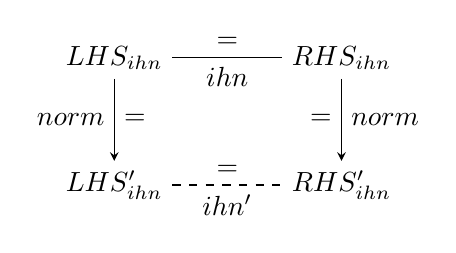
\begin{tikzpicture}
  \matrix (m) [matrix of math nodes,row sep=3em,column sep=4em,minimum width=2em]
  {
     LHS_{ihn} & RHS_{ihn} \\
     LHS'_{ihn} & RHS'_{ihn} \\};
  \path
    (m-1-1) edge [-stealth] node [left] {$norm$}
    						node [right] {$=$} (m-2-1)
            
    (m-1-1.east|-m-1-2) edge node [above] {$=$} 
    						 node [below] {$ihn$} (m-1-2)
    						 
    (m-2-1.east|-m-2-2) edge [dashed,-] node [above] {$=$}
										node [below] {$ihn'$} (m-2-2) 
    
    (m-1-2) edge [-stealth] node [right] {$norm$}
    						node [left] {$=$} (m-2-2);  
\end{tikzpicture}
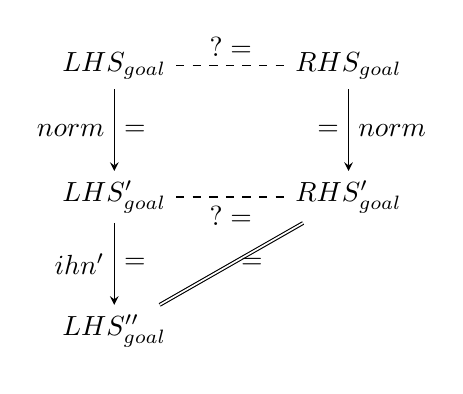
\begin{tikzpicture}
  \matrix (m) [matrix of math nodes,row sep=3em,column sep=4em,minimum width=2em]
  {
     LHS_{goal} & RHS_{goal} \\
     LHS'_{goal} & RHS'_{goal} \\
     LHS''_{goal} \\};
  \path
    (m-1-1) edge [-stealth] node [left] {$norm$}
							node [right] {$=$} (m-2-1)    
    
            edge [dashed,-] node [above] {$?=$} (m-1-2)

    (m-2-1.east|-m-2-2) edge [dashed,-] node [below] {$?=$} (m-2-2)
    (m-2-1) edge [-stealth] node [left] {$ihn'$}
							node [right] {$=$} (m-3-1)  
    
    (m-1-2) edge [-stealth] node [left] {$=$}  
							node [right] {$norm$} (m-2-2)
    
    (m-3-1) edge [double] node [right] {$=$} (m-2-2);    
\end{tikzpicture}

This example was a bit unconventional in the sense that 4 calls to the normalisation function were needed. Usually, only two calls to the normalisation are enough, one for the left hand side and one for the right hand side, and they are done in the decision procedure $commutativeMonoidDecideEq$. These two extra calls were needed because of the known equality that we had from the induction hypothesis. This example\footnote{Which can be found in $RingIdris/Examples/binary.idr$}, which was therefore at the boundary to deduction modulo [REF], shows that our implementation can deal with concrete goals obtained during the development of real programs.



\section {Discussion}

\label{sect:discuss}

	\subsection{An alternative approach, more traditional}

Without our type-safe reflection mechanism, the traditional way to go for this problem would be to have functions doing only computations, and some external lemmas about them. It would start with the definition of the function $reify\ :\ Expr\ \rightarrow\ c$. As we did in our approach, there would still be a function for reflecting terms $reflect\ :\ c\ \rightarrow\ Expr$. Because $reflect$ is a function based on syntax, it needs to use Idris' reflection mechanism. We would need to prove the correctness of these two functions, and it turns out that one lemma is enough for completely specifying the expected behaviour of these two functions at the same time : $reflect\_and\_reify\_correct\ :\ \forall\ x:c,\ reify\ (reflect\ x)\  \simeq \ x$.

Then comes the normalisation function : $normalize\ :\ Expr\ \rightarrow\ Expr$. Because this function is weekly typed compared to our approach (we no longer have an index giving a guarantee about the concrete values), we would need to provide a lemma of correctness about it after its definition. This lemma of correctness must say that the interpretation of the original (reflected) term is equal to the interpretation of the normalised (reflected) term. $normalize\_correct\ :\ \forall\ e:Expr,\ reify\ (normalize\ e)\  \simeq\ reify\ e$. We have avoided the need of such a --complicated-- proof in our correct by construction approach enabled by our type-safe reflection mechanism.

Now, similarly to what we've done, we would need a syntactical equality test, checking whether two reflected expressions are syntactically equal. The difference here is that, as often with this kind of "traditional" approach, we would produce something that belongs to the world of computations, usually a (pretty uninformative) boolean.
$beq_{Expr}\ :\ Expr\ \rightarrow\ Expr\ \rightarrow\ bool$. Because this boolean on its own is pretty uninformative, we now need a proof of correctness for this function as well, which says that if this function decides that two given terms are syntactically equal, then their interpretation should also be (syntactically) equal. $beq_{Expr}\_correct\ :\ \forall (e1\ e2:Expr), beq_{Expr}\ e1\ e2\ =\ true\ \rightarrow\ reify\ e1\  \simeq\ reify\ e2$. We did not have to do this proof either with our approach.

We could now build the kernel of the tactic, which is the following decision procedure. 
\begin{figure}[H]
\figrule
\begin{center}
\begin{lstlisting}
decideEq : c $\rightarrow$ c $\rightarrow$ bool 
decideEq x y =
      let ex = reflect x in 
      let ey = reflect y in
      $beq_{Expr}$ (normalise ex) (normalise ey)
\end{lstlisting}
\end{center}
\caption{Decision procedure of the tactic with a "traditional" approach}
\label{decideEqTrad}
\figrule
\end{figure}
This function on its own would not  be enough. We would need to add a correctness theorem, and this is precisely this main theorem that would help us to build the tactic we want.	
$decideEq\_correct\ :\ \forall\  x\ y:c,\ decideEq\ x\ y\ =\ true\ \rightarrow\ x\  \simeq\ y$. This proof can can made by combining, in this order, the three lemmas $beq_{Expr}\_correct$, $normalize\_correct$ (two times, one on each side of the assumed equality), and finally $reflect\_and\_reify\_correct$ (again two times).

Now, the tactic could be built by using this correctness theorem. When trying to prove a goal $a\ \simeq \ b$, the tactic would apply this theorem $decideEq\_correct$, which means that $x$ will be unified to $a$ and $y$ to $b$. The desired proof is thus produced if the premise $decideEq\ a\ b\ =\ true$ holds. But whether this premise holds or not can simply be tested by running the function $decideEq$ on the two arguments $a$ and $b$. 

Both with this ``traditional" approach and with our type-safe reflection, the activity of proving has effectively been replaced by the task of running a function, and a simple evaluation is now enough to produce the desired proof. The main advantage of our approach compared to this kind of traditional approach is that we don't need external lemmas, and more generally that the proof of correctness is obtained a lot more easily. Let's now see the differences more precisely with an actual implementation that almost follows the paradigm of the traditional approach.

	\subsection {Comparison with Coq's approach}
	
		\subsubsection{Description of Coq's implementation}	
	
In Coq's latest implementation of a Ring solver, described in~\cite{Coq2005}, they almost followed what has just been desribed as a ``traditional" approach with the use of many auxiliary lemmas. The few differences essentially lie in the way the function $reflect$ is defined. In Coq, they use the language LTac to program this automatic reflection\footnote{This function --that they call mkPolexpr-- can be found in $plugins/ring/Ring\_tac.v$}. Ltac is an untyped tactic language. It is untyped in the sense that an Ltac "function" produces something which might not have a valid  --and unique-- type. Because of this, Ltac definitions can only be used in the context of goals. Thus, applying a tactic defined with LTac might work, and then it makes progress to the current goal, or it might fail, and in this case the goal is kept unchanged. And anyway, the safety of the proof done is going to be checked during the final QED. So, Ltac functions can't be used in the statement of a lemma, and it is therefore not possible to reason about them. That means that it is not possible to write the lemma $reflect\_and\_reify\_correct$ of the "traditional" approach described in the previous subsection, because it is even impossible to state it as it uses a function defined in LTac. Because they can't even state this property, they can't finish the proof of the main theorem $decideEq\_correct\ :\ \forall\  x\ y:c,\ decideEq\ x\ y\ =\ true\ \rightarrow\ x \simeq\ y$. Indeed, the last step of this proof was to apply two times --one for the LHS, one for the RHS-- the fact that $\forall\ x:c,\ reify\ (reflect\ x)\ \simeq\ x$. One possibility would have been to add this axiom, but this is particularly unsightly, and potentially harmful. Also, it would imply that anyone using the ring prover would have this axiom added to his development, and would be forced to believe in it. Some proofs would be done automatically for the user of the system, but at the overly-expensive price of adding some uncertainty.
Instead, what they did for Coq's implementation of the Ring prover was to replace the main theorem $\forall\  x\ y:c,\ decideEq\ x\ y\ =\ true\ \rightarrow\ x\ \simeq\ y$ by the following weaker --but still powerful enough to build the desired tactic-- lemma\footnote{This lemma --that they call $setpolynomial\_simplify\_ok$-- can be found in $plugins/ring/Setoid\_ring\_normalize.v$}  : $f\_correct\ :\ \forall\ (e1\ e2\ :\ Expr),\ beq_{Expr}\ (norm\ e1)\ (norm\ e2)\ =\ true\ \rightarrow\ reify\ e1\ \simeq\ reify\ e2$.
Now, the tactic works like this. When trying to prove the goal $a \simeq b$, it computes $(reflect\ a)$ and $(reflect\ b)$. It then tries to apply $(f\_correct\ (reflect\ a)\ (reflect\ b))$ to the goal. 
\itemize
\item
If it can unify the goal $a \simeq b$ with $reify\ (reflect\ a)\ \simeq\ reify\ (reflect\ b)$ then it only has to check the validity of the premise by running the decision procedure. More precisely, if $beq_{Expr}\ (norm\ (reflect\ a))\ (norm\ (reflect\ b))$ is evaluated to $true$, then it has built the premise of $f\_correct$ and there's nothing left to prove. However, if the result was false, then it means that the automatic ring prover hasn't been able to prove this goal, because the LHS and RHS don't reduce to the same thing. If this ring prover is complete, it means that $a$ is not\footnote{Note that in this case, it hasn't produced such a formal proof of disequality, which isn't the goal of a ring prover} equal to $b$, or at least, they aren't equal only with the properties of a ring.
\item
if it couldn't unify the goal $a \simeq b$ with $reify\ (reflect\ a)\ \simeq\ reify\ (reflect\ b)$, then it means that there is something wrong in the definitions of the functions $reflect$ and $reify$, and it could print something like ``The ring prover has failed unexpectedly. There's something wrong with the implementations of the $reflect$ and $reify$ functions". Nothing really bad happened, as no inconsistent proof has been produced, nor no axioms added. That would just mean that the implementation of the ring prover is slightly broken, and that some goals that should be automatically provable aren't automatically proved. Thus, it would only decrease the completeness of the prover. That would be of course bad --because in the extreme case, the prover never succeeds in a generating a proof and is thus completely useless--, but that would only limit the scope of usage of the prover. \\

		\subsubsection{Differences with Coq's implementation}

Coq's ring prover follows the traditional\footnote{By ``traditional" we have in mind the proof engineering style developed in the Coq'Art ~\cite{BertotC04}}  approach of defining functions, and latter on proving many auxiliary lemmas about them. This is particularly adapted to Coq, which has many facilities for the construction of proofs, and a powerful proof mode. However, this approach kind of duplicate the work : they first tell the machine how it works, and latter, why it works. This separation between the world of computations and the world of logic becomes smaller in our approach with a fine use of dependent types, that allows to write more specific types, and thus to capture logical properties. The writing of functions can therefore be guided by this more precise type, and this is one of the main benefit of the approach we've followed. Moreover, we almost get the proof of correctness for free, because every little bit of rewriting done for the normalisation of the reflected terms is accompanied by the logic justification which tells why this rewriting can be done --and locally, this justification is always simple !--. In the end, all the proofs we have to do are systematically straightforward, since they only contain rewritings with the available hypothesis and the use of the properties of the corresponding algebraic structure. \\

Another difference with our implementation is that we've implemented a hierachy of tactics for many algebraic structures, but Coq's implementation only deals with ring and semi ring. If someone wants to prove equalities in a commutative group that isn't a ring, he simply can't use their prover. A dedicated prover for commutative groups would be needed, and Coq currently doesn't has one. The worst is that such a prover for commutative group would do very similar treatments, which means a lot of code could have been factorised. This is what we've obtained by taking this in account from the start. Our monoid prover used the underneath semi-group prover, our group prover uses the underneath monoid prover, and so on. \\

In terms of performances, our implementation is fast enough for providing answers in a decent amont of time --usually a few seconds--. For example, the automatic proof of the lemma $adc\_lemma\_2$ (presented in section~\ref{sect:motivatingExample} and proven automatically in section ~\ref{sect:results}) is constantly generated and printed in less than 8 seconds on a dual core i5 processor @ 2.4ghz and is therefore perfectly usable, even for this kind of moderate to large size proofs that come from a real application. Knowing that the display of the proof takes most of the time, it would be interesting to evaluate precisely the time needed for its generation only, without outputting the result. However, we suspect that our implementation will be slower than Coq, because they've used a more efficient representation of normalised polynomials. It might be possible that we've traded some efficiency against some simplicity and compositionality of the various provers.

	\subsection{Other related work}
	
As mentioned, Coq's implementation of a ring prover was also using proof-by-reflection techniques, but without the guarantees obtained with our type-safe reflection mechanism. Their automatic reflection is programmed in Ltac~\cite{DelahayeLTac} : a proof dedicated and untyped meta-language for the writing of automations. Because $Ltac$ is untyped, it would not permit to define --as we did-- a dependently typed function $reflect$ that is guaranteed to return a faithful encoding of the given input value. $Mtac$~\cite{Ziliani13} is an extension to Coq that supports dependently-typed tactic programming, which uses monad to avoid the need to touch the trusted kernel typechecker of Coq.
\\

Doing proofs by reflection has been intensively investigated by many authors, including Adam Chlipala, in particular in his book~\cite{ChlipalaBook} and in~\cite{Malecha14}. However, we haven't found anything similar to the type-safe reflection technique that we've presented in this paper. 
\\

At the connexion bewteen proof automation and proof by reflection, we can cite SSreflect~\cite{GonthierTuto}, which is an extension of Coq which aims to provide additional formalisations and tactics suitable for long mathematical proofs.
\\

Proof automation has been investigated for various proof assistants and programming languages. In Coq, appart from the $ring$ prover~\cite{Coq2005}, there's also the $omega$ solver~\cite{Cregut04}, which solves a goal in Presburger arithmetic (i.e. a universally quantified formula made of equations and inequations), and a Field~\cite{DelahayeField} decision procedure for real numbers, which plugs to Coq's ring prover after simplification of the multiplicative inverses. Various automations have also been done in Agda~\cite{Lindblad04}.
\\

Finally, when we leave the ground of nice mathematical structures (like groups, rings and fields), one can decide to work with arbitrary rewriting rules, but in the general case there isn't a complete decision procedure for such problems, because there's usually no normal form. This is where deduction modulo~\cite{Dowek03} ~\cite{DelahayeModulo} starts.


	\subsection {Correctness and completeness}

		\subsubsection{Correctness}
		
The correctness of all of our tactics is in fact obtained by construction. Actually, what we really needed to produce was the proof of the equality $a \simeq b$, and not the normalised terms. The normalised term --and more precisely their construction-- was just a support for building the desired proof of $a \simeq b$, which is precisely the proof of correctness. Thus, there isn't any possibility that we've generated a wrong proof as long as we ensure that :
\begin{itemize}
\item We haven't introduced any axioms
\item We haven't introduced any non total\footnote{Contrary to Coq, Idris allows the definition of non-total functions for helping the development of non-finished real-world projects} function or proof used for the building of the main proof $a \simeq b$. Note that the normalization itself could contain some non total functions without breaking the correctness. That would just mean that when using this tactic, the tactic could potentially loop infinitely and the user would never get his answer. That would of course be bad, but that would not produce any inconsistency --as long as none uses these definitions maliciously to prove something false--, because this non total function would be only used in the world of computations and not in the world of logic.
\end{itemize}

Because we've meet these two conditions, we simply can't produce a false proof of a statement, because the typechecker would complain if that would be the case. If Idris internal type theory is consistent and if Idris' internal implementation follows it (and we believe in both!), then one can't produce a false lemma without either introducing an axiom nor introducing a non total function and latter using it maliciously to create an inconsistency in the logic.

		
		\subsubsection{Completeness}
		
Completeness means that when given an equality which is provable by using the properties of the concerned algebraic structure, the adapted prover should be able to generate a proof of this equality. Having a complete tactic is important, because otherwise the tactic is not always usuable -- and in the worst case it is never usable--, and thus is not really valuable. However, having a formal proof of the completeness in the system itself isn't really interesting. As long as we do not meet an equality that should be provable, and which isn't proved by our tactic, there is no problem. And if this situation does happen one day, nothing really bad happened : no inconsistencies would have been introduced in the system. The tactic would just refuse to do it automatically, but the user could still attempt it. \\

In definitive, we want the tactic to be complete, without requiring a formal proof of it. If we believe that the normal form computed by the reduction function is indeed a normal form --which means that if two terms are equal according to the properties of the algebraic structure, then their normal form should be equal-- then the tactic is complete.
Indeed, 
$isNormalForm\ :\ \forall\ a\ b,\ a \simeq b \rightarrow norm\ (reflect\ a) = norm\ (reflect\ b)$ is logically equivalent to

$completeness : \ \forall\ a\ b,\ norm\ (reflect\ a) \neq norm(reflect\ b) \rightarrow a \not{\simeq} b$, which is in fact :
$\ \forall\ a\ b,\ decideEq\ (reflect\ a)\ (reflect\ b) = Nothing \rightarrow a \not{\simeq} b$.
This equivalence between $isNormalForm$ and $completeness$ can only be done in the meta theory because it is a proof by contradiction, which is equivalent to the law of excluded middle, that we do not have in constructive logics, on which Idris is based.
\\

So far, we haven't encountered any goal that should be provable but which failed to be proven automatically. However, if this situation would appear one day, it would certainly come from a small kind of simplification that would have been forgotten somewhere in the hierarchy, and it would be easy to fix it by adding a sub-function that deals with this specific simplification at the appropriated level. All the more specialised provers that reuse this prover would also be fixed at the same time thanks to the compositionality of our provers. 
\\

Another little advantage of our approach is that we have the guarantee that we can't lose any totality because of the $reflect$ function. The reason is that the produced reflected term is indexed over the original --concrete-- value. By this fact, we don't need a $reify$ function. If we want to go from the reflected term to the original --concrete-- value, we can simply return the index. Thus, unlike Coq, we have the formal guarantee that $(reflect\ a)$ is always a faithful representation of $a$ with our approach, which means that we can't lose any totality because of the $reflect$ function.


	\subsection {Conclusion and futur work}
	
This paper has shown that type-safe reflection techniques can enable to manipulate proofs terms easily. We've been able to build an entire hierarchy of tactics for algebraic structures precisely because the construction of the proof terms has been greatly facilitated by the use of this technique. We end up with a hierarchy of reflexive tactics for proving equivalence in semigroups, monoids, commutative monoids, groups, commutative groups, pre semi-ring, semi-ring, rings and commutative rings, without having had to repeat our efforts.

It is even possible to extend a prover in order to build a dedicated one for a specific structure that isn't exactly a well known algebraic structure. We are at the moment investigating the extention of the pre semi-ring prover in order to build a prover for regular expressions. Regular expressions have a union of language playing the role of $+$ (which is associative, commutative, and which has a neutral element $\emptyset$) and a product of language playing the role of $*$, which is associative, distributive over the union, and which admits the empty word $\epsilon$ for neutral element. However, it has also a Kleene $star$ construction and a few properties about it. We currently aim to extend the pre semi-ring prover in order to build a prover for regular expression. Such a prover would be useful for doing formally-verified-for-free transformations of regular grammars and final states machines, which could go up to a formally verified (for free!) parser generator for regular languages.





\bibliographystyle{jfp}
\bibliography{dtp}

%\begin{thebibliography}{}
% \bibitem[\protect\citename{B. Gregoire and A. Mahboubi}2005]{Coq2005}
%   Gregoire,~B. and Mahboubi,~A. (2005) Proving equalities in a commutative ring done right in Coq, TPHOLs 2005, Oxford, UK, August 22-25, 2005, Proceedings


% \bibitem[\protect\citename{W.A Howard}1980]{How80}
%   Howard W.A. The formulae-as-types notion of construction. In J. R. Seldin and J. P. Hindley, editors, To H. B. Curry: Essays on Combinaory Logic, Lambda Calculus, and Formalism. Academic Press, 1980.


%\end{thebibliography}

\end{document}

% end of JFP2egui.tex

